\begin{figure*}[!t]
	\begin{minipage}[t]{0.48\linewidth}
		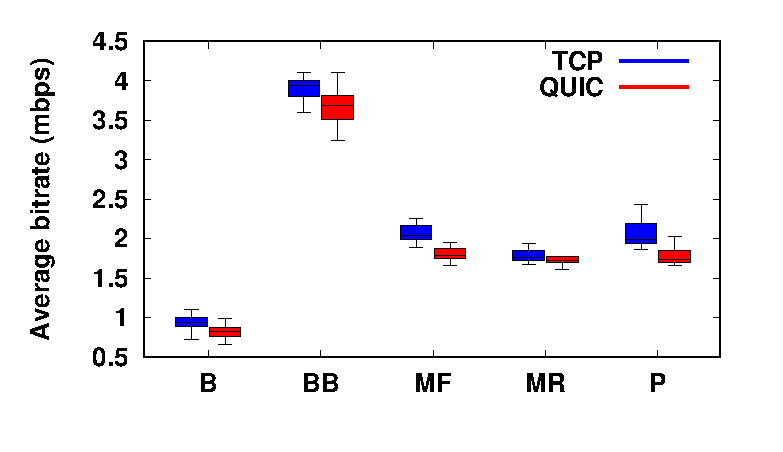
\includegraphics[width=\linewidth]{img/newexp/bitrate_box}
		\caption{\label{fig:averageQuality_n}Average Playback Video Quality for Different ABR Techniques ($p<0.05$ for all the metrics)}
	\end{minipage}\hfill
	\begin{minipage}[t]{0.48\linewidth}
		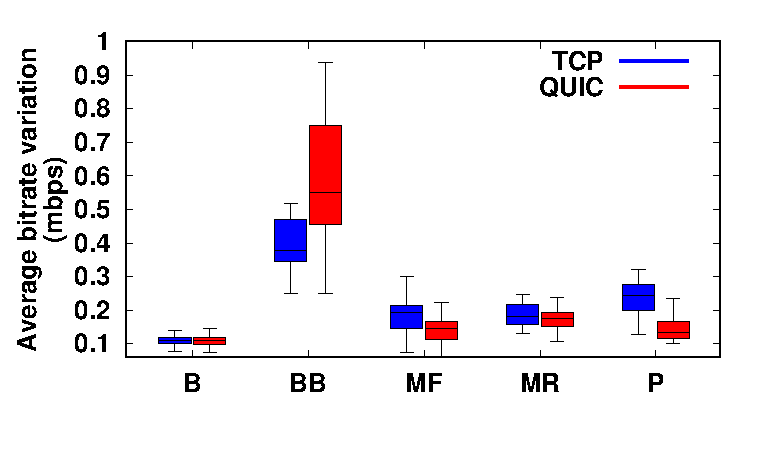
\includegraphics[width=\linewidth]{img/newexp/smooth_box}
		\caption{\label{fig:averageQualityVariation_n}Average Playback Quality Variation for Different ABR Techniques ($p<0.05$ for all the metrics except BOLA and MPC-Robust)}
	\end{minipage}\hfill
	\begin{minipage}[t]{0.48\linewidth}
		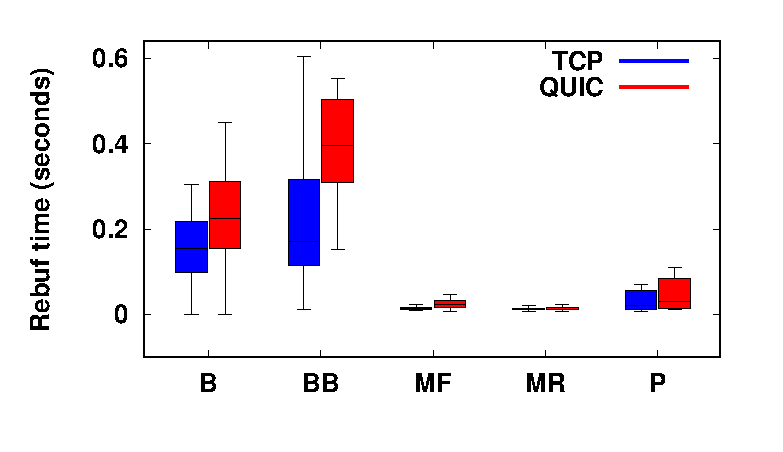
\includegraphics[width=\linewidth]{img/newexp/rebuf_box}
		\caption{\label{fig:RebufferTime_n}Rebuffering Time for Different ABR Techniques ($p<0.05$ for all the metrics except Pensieve and MPC-Robust)}
	\end{minipage}\hfill
	\begin{minipage}[t]{0.48\linewidth}
		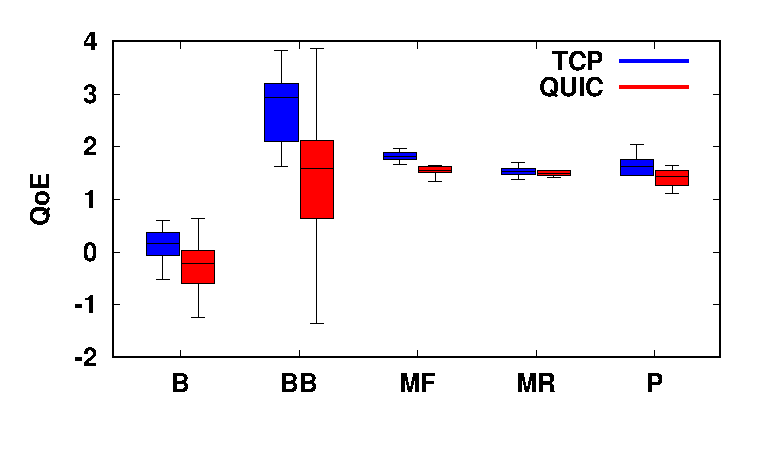
\includegraphics[width=\linewidth]{img/newexp/qoe_box}
		\caption{\label{fig:QOE_n}Overall QoE for Different ABR Techniques ($p<0.05$ for all the metrics except MPC-Robust)}
	\end{minipage}
\end{figure*}

%\begin{figure*}
%	\captionsetup[subfigure]{}
%	\begin{center}
%		\subfloat[\label{fig:averageQuality_n}]{
%			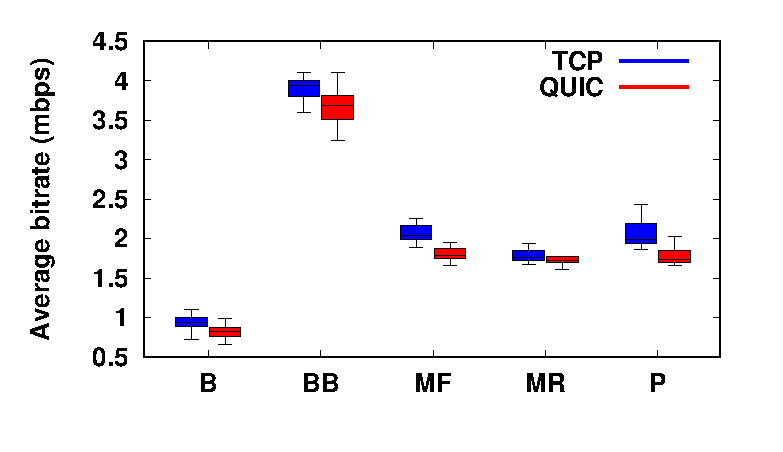
\includegraphics[width=.24\linewidth]{img/newexp/bitrate_box}
%		}
%		\subfloat[\label{fig:averageQualityVariation_n}]{
%			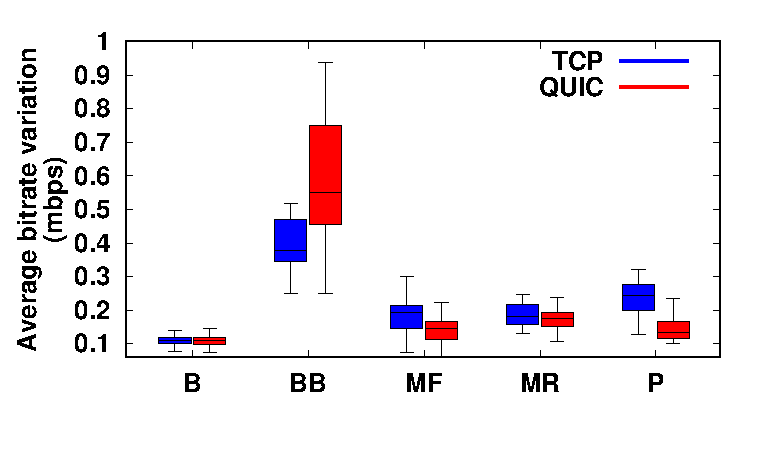
\includegraphics[width=.24\linewidth]{img/newexp/smooth_box}
%		}
%		\subfloat[\label{fig:RebufferTime_n}]{
%			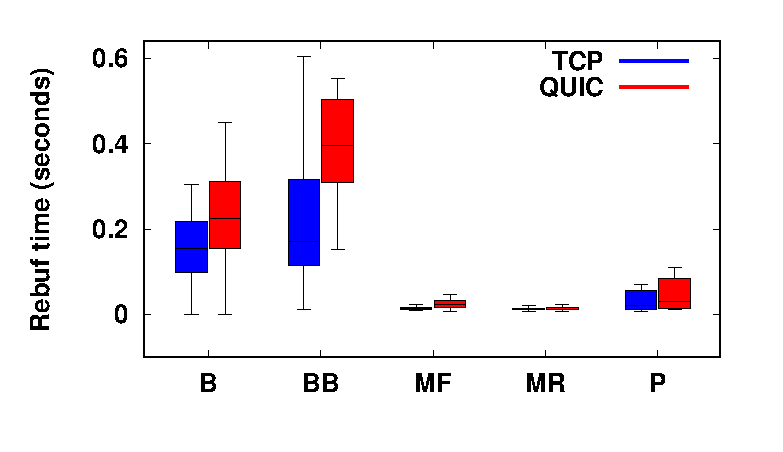
\includegraphics[width=.24\linewidth]{img/newexp/rebuf_box}
%		}
%		\subfloat[\label{fig:QOE_n}]{
%			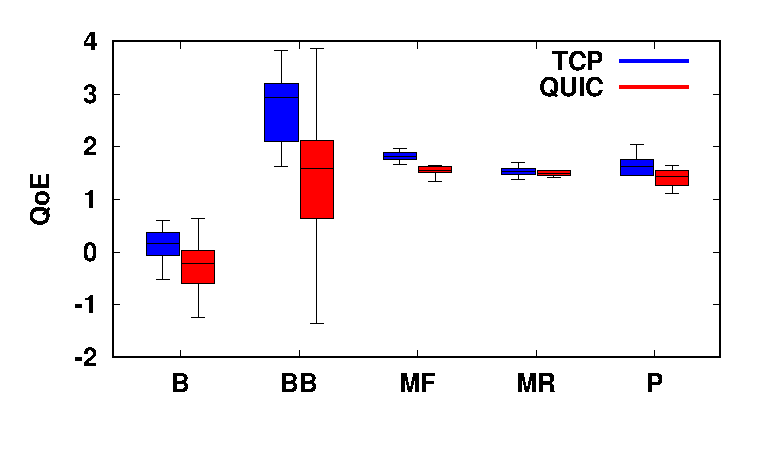
\includegraphics[width=.24\linewidth]{img/newexp/qoe_box}
%		}
%	\end{center}
%	\caption{\label{fig:qoe_comp}(a) Average Playback Video Quality for Different ABR Techniques ($p<0.05$ for all the metrics), (b) Average Playback Quality Variation for Different ABR Techniques ($p<0.05$ for all the metrics except BOLA and MPC-Robust), (c) Rebuffering Time for Different ABR Techniques ($p<0.05$ for all the metrics except Pensieve and MPC-Robust) and (d) Overall QoE for Different ABR Techniques ($p<0.05$ for all the metrics except MPC-Robust)}
%\end{figure*}

\section{Results and Analysis}
%We have plotted our findings in Fig.~\ref{fig:averageQualityVariation}, \ref{fig:averageQuality}, \ref{fig:QOE}, \ref{fig:RebufferTime} and \ref{fig:StartupDelay}. We run the wilcoxon rank-sum test on the data (which are significant) to avoid any statistical assumptions.
%In this section, we look into the detailed performance comparison of QUIC and TCP in terms of DASH QoE metrics as discussed in the previous section. 
We first look into the overall playback video quality and then dig into the details of individual QoE metrics. \blue{As the data used for this analysis have been collected from realistic experiments, we, therefore, avoid any underlying parametric assumption while checking for the statistical significance of the results. Subsequently, we apply Mann–Whitney U test~\cite{mannwhitney} with non-parametric assumptions on all the metrics and report if the results are statistically significant or not with the hypothesis that DASH/TCP works significantly better than DASH/QUIC\footnote{\blue{We use the notation ``DASH/TCP'' to indicate DASH over TCP; similarly ``DASH/QUIC'' indicates DASH over QUIC.}}. We also run a two-way test to check the alternate hypothesis that DASH/QUIC works significantly better than DASH/TCP.}

%\begin{figure}
%	\captionsetup[subfigure]{}
%	\begin{center}
%		\subfloat[\label{fig:averageQuality}]{
%			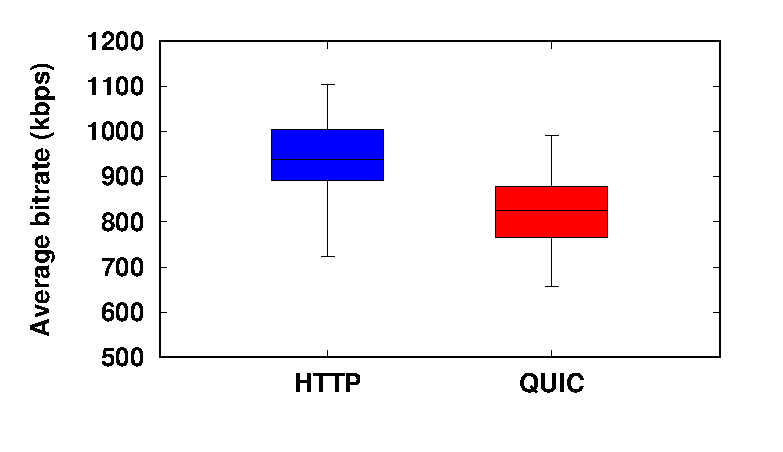
\includegraphics[width=.49\linewidth]{img/exp/AQ_box}
%		}
%		\subfloat[\label{fig:averageQuality_n}]{
%			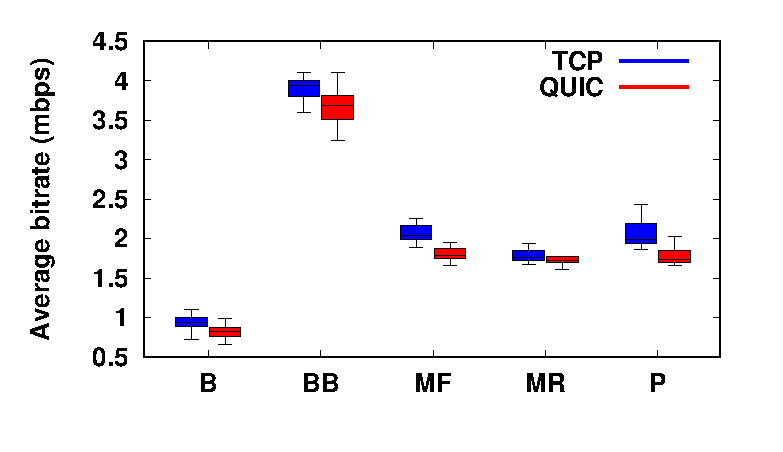
\includegraphics[width=.49\linewidth]{img/newexp/bitrate_box}
%		}
%	\end{center}
%	\caption{\label{fig:aq}(a) Average Playback Video Quality, (b) Average Playback Video Quality for Different ABR Techniques ($p < 0.05$ for all the metrics)}
%\end{figure}



\subsection{Average Video Bitrate}
%(RanksumsResult(statistic=-5.510617155085412, pvalue=3.5757771447496305e-08))
%We first observe the average playback video quality with the default DASHIF ABR technique %BOLA(B)~\cite{bola-2016} which uses the playback buffer occupancy as an indicator of the quality level adaptation. Fig.~\ref{fig:averageQuality_n} shows a comparison between HTTP over TCP and HTTP over QUIC in terms of average video playback quality (bitrate) with BOLA as the bitrate adaptation mechanism. 
%\noteam{Mannwhitneyu test with non-parametric assumptions}
%\begin{figure}
%	\captionsetup[subfigure]{}
%	\begin{center}
%		\subfloat[\label{fig:averageQuality_box_n}]{
%			\includegraphics[width=.49\linewidth]{}
%		}
%		\subfloat[\label{fig:averageQuality_cmf_n}]{
%			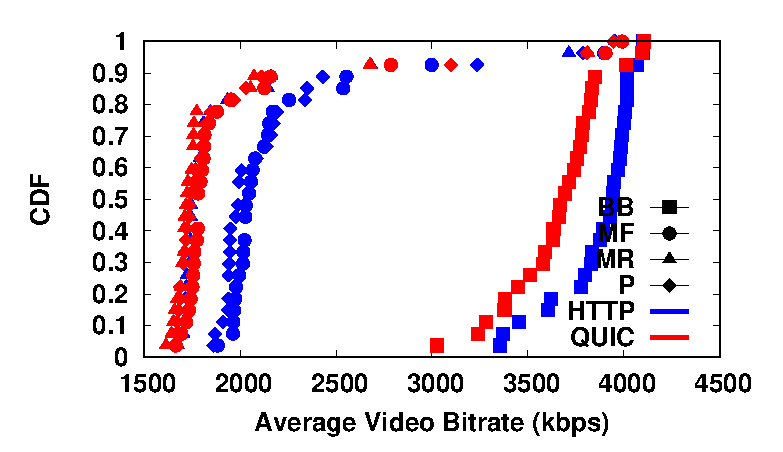
\includegraphics[width=.49\linewidth]{img/newexp/bitrate_cdf}
%		}
%	\end{center}
%	\caption{\label{} }
%\end{figure}
%We first look into the average playback quality for different ABR mechanisms such as BOLA (B), buffer based (BB), MPC-Fast (MF), MPC-Robust (MR) and Pensieve. 
The distributions of the average playback bitrate for the five ABR mechanisms are shown in Fig.~\ref{fig:averageQuality_n}. For BOLA, we observe that the average video bitrate for DASH/TCP is higher than that of DASH/QUIC. It is known from the existing literature that buffer-based ABR mechanisms aggressively use the highest quality levels, which we also observe in Fig.~\ref{fig:averageQuality_n}. However, we observe that DASH/TCP always performs better than DASH/QUIC. Indeed, the state-of-the-art reinforcement learning based ABR mechanism, Pensieve, provides much better quality level on top of TCP in comparison to QUIC. \blue{For all the five ABR methods, we observe that the $p$-value is less than $0.05$ for the Mann–Whitney U test, indicating that DASH/TCP performs significantly better than DASH/QUIC in terms of average playback quality.} 
%This indicates that adaptive streaming works better over TCP compared to QUIC, when we consider the overall playback quality level. 
%Next, we explore other video QoE metrics. 

%At first we tried to observer the average playback quality for both the protocol. So, in Fig.~\ref{fig:averageQuality} we have potted the average playback quality in terms of bitrate. From figure we can see that we average quality is higher for HTTP than that of QUIC. The entire range of average bitrate is better for HTTP than QUIC. Maximum average bitrate for HTTP 1100kbps where QUIC is 900kbps.

%\begin{figure}
%	\captionsetup[subfigure]{}
%	\begin{center}
%		\subfloat[\label{fig:averageQualityVariation}]{
%			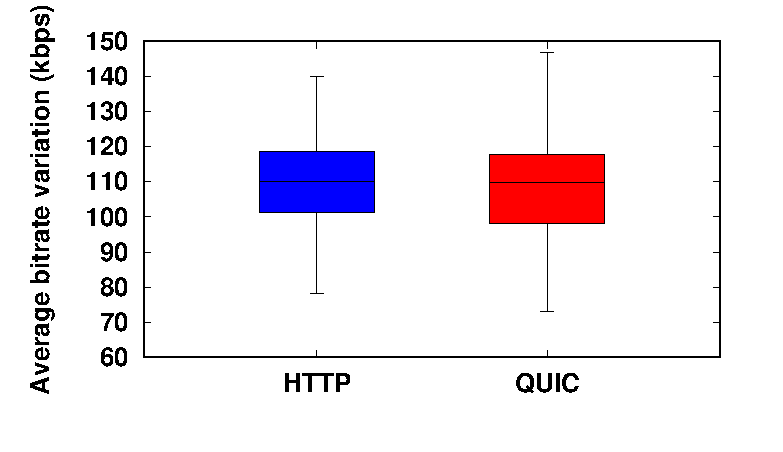
\includegraphics[width=.49\linewidth]{img/exp/AQV_box}
%		}
%		\subfloat[\label{fig:averageQualityVariation_n}]{
%			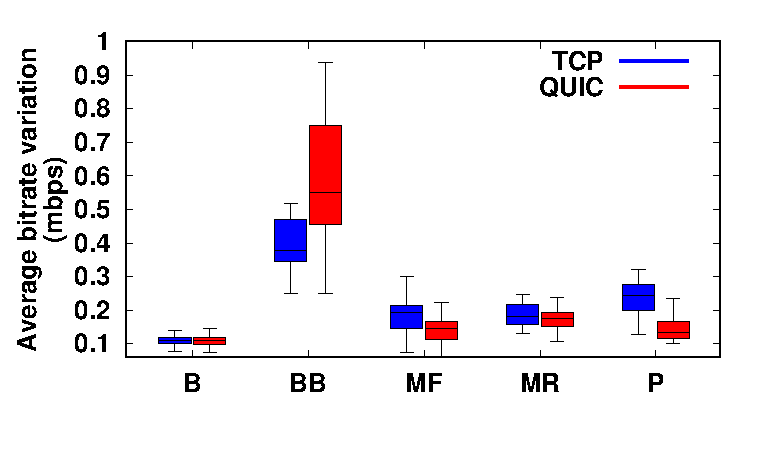
\includegraphics[width=.49\linewidth]{img/newexp/smooth_box}
%		}
%	\end{center}
%	\caption{(a) Average Playback Quality Variation, (b) Average Playback Quality Variation for Different ABR Techniques ($p < 0.05$ for all the metrics except Bola and MPC-Robust)}
%\end{figure}
%(RanksumsResult(statistic=0.4086028752267741, pvalue=0.6828311202973789))

%\begin{figure}
%	\captionsetup[subfigure]{}
%	\begin{center}
%		\subfloat[\label{fig:averageQualityVariation_box_n}]{
%			\includegraphics[width=.49\linewidth]{}
%		}
%		\subfloat[\label{fig:averageQualityVariation_cdf_n}]{
%			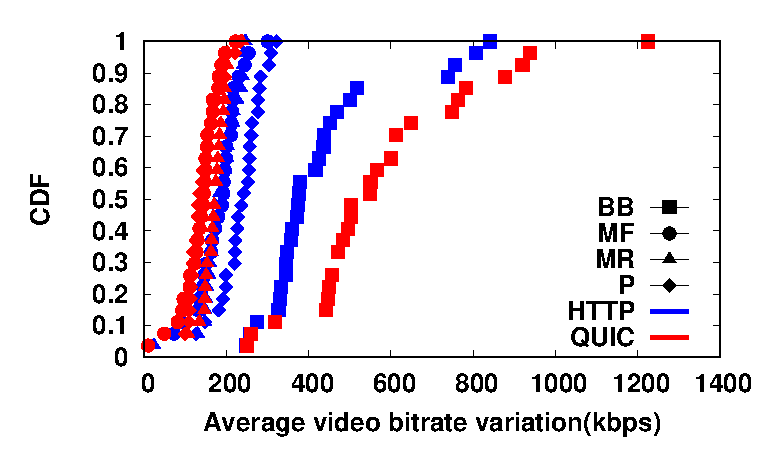
\includegraphics[width=.49\linewidth]{img/newexp/smooth_cdf}
%		}
%	\end{center}
%	\caption{\label{}}
%\end{figure}

\subsection{Quality Level Fluctuation -- Playback Smoothness}
%Average quality variation in terms of bitrate is almost same for HTTP and QUIC (Fig.~\ref{fig:averageQualityVariation}) although maximum and minimum variation is higher for QUIC. This variation reflect in QoE measurements.
Next, we observe the average fluctuation in the playback quality levels, which has been shown in Fig.~\ref{fig:averageQualityVariation_n}. A fluctuation in the quality level indicates less smoothness in the video playback, and, therefore, reduces the QoE. \blue{We observe that the differences in average quality level fluctuations between DASH/TCP and DASH/QUIC for BOLA and MPC-Robust are statistically insignificant. However, the figure indicates that quality fluctuation with DASH/QUIC is significantly more for buffer-based ABR, whereas less for MPC-Fast and Pensieve-based ABR, with $p$-value less than $0.05$.} This is an interesting observation as we see that the advanced ABR techniques, such as MPC\blue{-Fast} and Pensieve, provide better playback smoothness with DASH/QUIC, although the supported playback quality is lower compared to DASH/TCP. 

%\begin{figure}
%	\captionsetup[subfigure]{}
%	\begin{center}
%		\subfloat[\label{fig:RebufferTime}]{
%			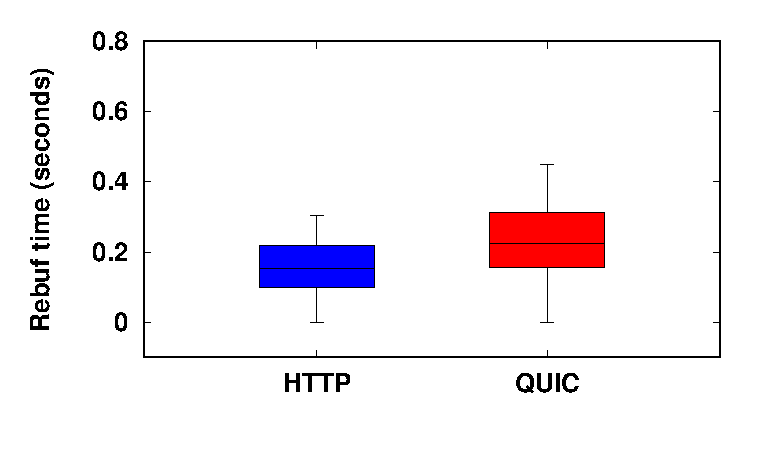
\includegraphics[width=.49\linewidth]{img/exp/RT_box}
%		}
%		\subfloat[\label{fig:RebufferTime_n}]{
%			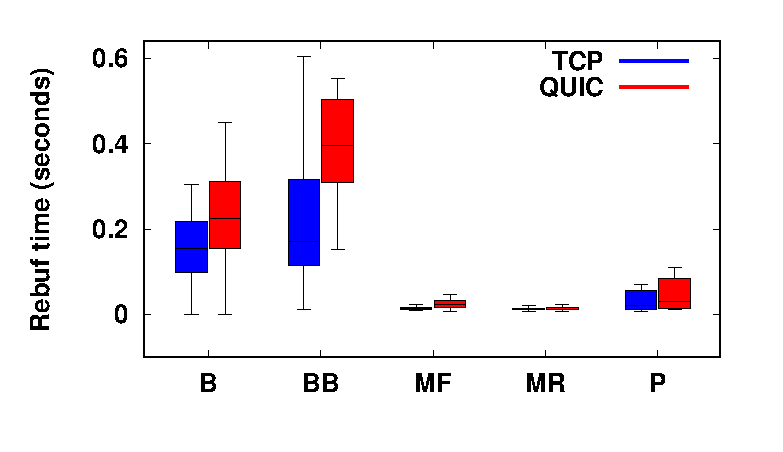
\includegraphics[width=.49\linewidth]{img/newexp/rebuf_box}
%		}
%	\end{center}
%	\caption{ (a) Rebuffering Time, (b) Rebuffering Time for Different ABR Techniques ($p < 0.05$ for all the metrics except Pensieve and MPC-Robust)}
%\end{figure}
%(RanksumsResult(statistic=-3.152868131817405, pvalue=0.0016167482331207014))

%
%\begin{figure}
%	\captionsetup[subfigure]{}
%	\begin{center}
%		\subfloat[\label{fig:RebufferTime_box}]{
%			\includegraphics[width=.49\linewidth]{}
%		}
%		\subfloat[\label{fig:RebufferTime_cdf_n}]{
%			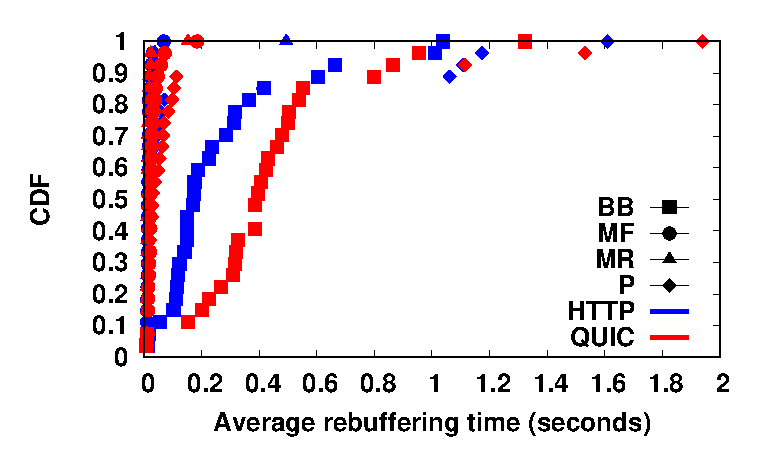
\includegraphics[width=.49\linewidth]{img/newexp/rebuf_cdf}
%		}
%	\end{center}
%	\caption{\label{} }
%\end{figure}

\subsection{Rebuffering Time}
%Next, we analyze one of the most important QoE metrics -- the rebuffering time. Most of the existing literature claims that the QoE drops significantly with a rebuffering during the video playback. 
Fig.~\ref{fig:RebufferTime_n} indicates the rebuffering time for different ABR techniques over DASH/TCP and DASH/QUIC. \blue{We observe that rebuffering is significantly more with DASH/QUIC for BOLA, buffer-based and MPC-Fast, whereas the differences in rebuffering are statistically insignificant for MPC-Robust and Pensieve}. For the buffer-based ABR which aggressively download the videos at the highest playback quality, rebuffering is comparatively very high with DASH/QUIC. \blue{MPC-Robust and Pensieve show minimal rebuffering, so the differences between DASH/TCP and DASH/QUIC are not statistically significant.} We observe that the claim from Google~\cite{langley2017quic} that QUIC enables less rebuffering does not hold for all the ABR techniques and is very much specific to which ABR technique is adopted at the playback client.  

%\begin{figure}
%	\captionsetup[subfigure]{}
%	\begin{center}
%		\subfloat[\label{fig:QOE}]{
%			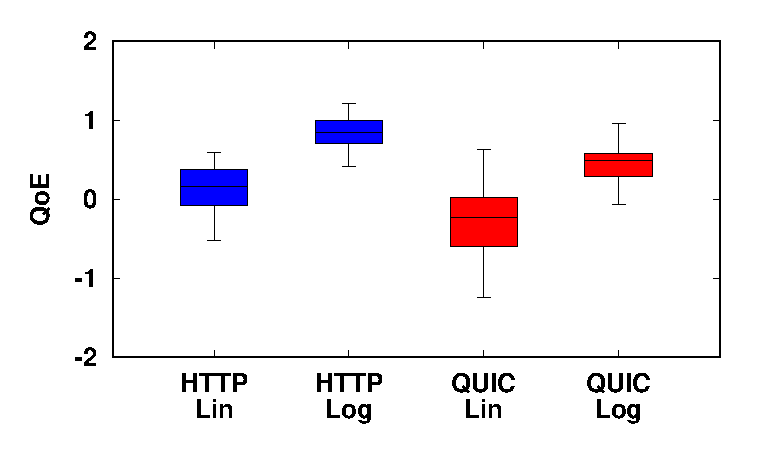
\includegraphics[width=.49\linewidth]{img/exp/QOE_box}
%		}
%		\subfloat[\label{fig:QOE_n}]{
%			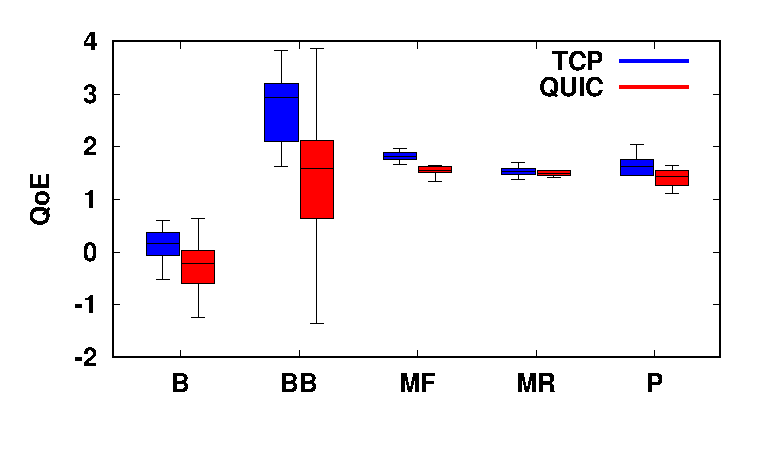
\includegraphics[width=.49\linewidth]{img/newexp/qoe_box}
%		}
%	\end{center}
%	\caption{\label{fig:aqoe}(a) Overall QoE, (b) Overall QoE for Different ABR Techniques ($p < 0.05$ for all the metrics except MPC-Robust)}
%\end{figure}
%(lin: RanksumsResult(statistic=2.4626605723127195, pvalue=0.013791040475998067), log: RanksumsResult(statistic=4.052898789411516, pvalue=5.058689107127597e-05))

%\begin{figure}
%	\captionsetup[subfigure]{}
%	\begin{center}
%		\subfloat[\label{fig:QOE_box_n}]{
%			\includegraphics[width=.49\linewidth]{}
%		}
%		\subfloat[\label{fig:QOE_cdf_n}]{
%			\includegraphics[width=.49\linewidth]{}
%		}
%	\end{center}
%	\caption{}
%\end{figure}

\subsection{Overall QoE}
Finally, we look into the overall QoE computation as shown in Eq.~(\ref{eqn:QoE}). The overall QoE measurements for  all the ABR techniques are shown in Fig.~\ref{fig:QOE_n}. In this experiment, we plot the linear variants of $q(R_n)$ as discussed in the previous section. Our observations from these results are as follows. \blue{DASH/TCP provides significantly better QoE compared to DASH/QUIC for all the ABR algorithms except MPC-Robust where the result is statistically insignificant.} This indicates that the recent advanced ABR techniques like MPC and Pensieve are more compatible with TCP than QUIC. Indeed from representations of $q(R_n)$, we can say that the above observations are generic across a wide variation of QoE measurements. 


